\chapter{Implantação e hospedagem}
\label{chap:implantacao}

Este capítulo descreve a infraestrutura usada para disponibilizar o FlashFood, as funções da máquina virtual e do servidor próprio e a comunicação entre os componentes da aplicação.

\section{Infraestrutura de hospedagem}

A hospedagem do FlashFood utilizou dois equipamentos com funções distintas: uma máquina virtual contratada na HostGator e o servidor próprio do projeto. A máquina virtual forneceu um endereço IP fixo utilizado para o acesso externo ao sistema. A aplicação Laravel e o banco de dados MySQL permaneceram em execução no servidor próprio; portanto, a máquina virtual não armazenava os dados da aplicação nem executava sua lógica de negócio.

O endereço utilizado para acessar o sistema pelo navegador é \url{https://www.flashfood.store/}. A disponibilidade da aplicação nesse domínio depende do redirecionamento do tráfego na máquina virtual para o servidor próprio pelo túnel WireGuard. Quando esse redirecionamento está desativado, o sistema não fica acessível pelo domínio.

A escolha do plano com recursos reduzidos teve como objetivo diminuir o custo da disponibilização externa do sistema. Como a aplicação e o banco de dados eram executados no servidor próprio, não era necessário utilizar a máquina virtual para processamento ou armazenamento desses componentes. Para a arquitetura adotada, a função principal da VM era fornecer um endereço IP público fixo e atuar como ponto remoto da conexão WireGuard, pela qual o tráfego de acesso era encaminhado ao servidor do projeto. Na comparação de preços realizada pelo autor à época da contratação, esse plano apresentou custo inferior ao da contratação de um endereço IP fixo com um provedor de \textit{Internet} local. Assim, foi priorizada uma configuração de menor custo que atendesse ao requisito de acesso externo ao sistema.

\section{Recursos computacionais}

A Tabela~\ref{tab:recursos-hospedagem} resume as especificações informadas para os dois equipamentos. Os valores de memória representam a capacidade total indicada pelas ferramentas, e não o consumo momentâneo observado durante a coleta.

\begin{table}[htbp]
\centering
\caption{Recursos utilizados na hospedagem do sistema}
\label{tab:recursos-hospedagem}
\small
\begin{tabularx}{\textwidth}{p{3.1cm} X X}
\hline
\textbf{Equipamento} & \textbf{Especificações} & \textbf{Função na hospedagem} \\
\hline
Máquina virtual da HostGator & Plano VPS NVMe 2, com 1 vCPU, 2 GB de memória DDR5, 50 GB de armazenamento NVMe e um IP dedicado. O ambiente utiliza Ubuntu 22.04.5 LTS, \textit{kernel} Linux 6.8.0-138-generic e virtualização KVM/OpenStack. O sistema operacional reconhece 1,9 GiB de RAM e não possui área de troca (\textit{swap}) configurada. & Receber o acesso externo pelo IP fixo e participar da conexão VPN com o servidor próprio. \\
\hline
Servidor próprio & Computador \textit{desktop} com arquitetura x86-64, Ubuntu 24.04.5 LTS, \textit{kernel} Linux 6.8.0-147-generic, 15 GiB de memória RAM e 4 GiB de área de troca (\textit{swap}). & Executar a aplicação Laravel e o banco de dados MySQL. \\
\hline
\end{tabularx}
\legend{Elaborado pelo autor (2026)}
\end{table}

\section{Comunicação por meio do WireGuard}

A comunicação entre a máquina virtual e o servidor próprio foi estabelecida por meio de uma VPN configurada com WireGuard \cite{donenfeld2017wireguard}. Essa configuração criou uma rede privada entre os equipamentos, permitindo encaminhar o tráfego entre eles sem expor diretamente à \textit{Internet} os endereços utilizados nessa rede. Na configuração do servidor próprio, a interface WireGuard recebeu o endereço \texttt{10.200.200.2/24}. A faixa \texttt{10.200.200.0/24} foi indicada como rede acessível pelo túnel, e o \textit{peer} remoto foi configurado para ser alcançado pelo endereço público da máquina virtual na porta UDP \texttt{25000}.

Na VM, o Nginx escuta nas portas TCP \texttt{80} e \texttt{443}, enquanto o WireGuard recebe conexões na porta UDP \texttt{25000}. A configuração do Nginx contém blocos para os domínios \texttt{flashfood.store} e \texttt{www.flashfood.store}; o bloco HTTPS escuta na porta \texttt{443} com TLS e encaminha as requisições para \texttt{http://10.200.200.2:8000}. Dessa forma, o Nginx da VM atua como \textit{proxy} reverso e envia o tráfego ao servidor próprio pela rede WireGuard \cite{nginxBeginnersGuide}. O TLS é encerrado na VM, e a conexão HTTP entre os servidores percorre o túnel VPN. A saída das tabelas NAT não mostrou uma regra \texttt{DNAT} para esse fluxo, o que é compatível com o uso de \textit{proxy} reverso. O parâmetro \texttt{net.ipv4.ip\_forward=1} também está habilitado. Em um teste realizado localmente na VM, uma requisição HTTP para \texttt{www.flashfood.store} retornou o status \texttt{301 Moved Permanently} e o cabeçalho \texttt{Location: https://www.flashfood.store/}, confirmando o redirecionamento da porta \texttt{80} para HTTPS. A resposta também informou o servidor \texttt{nginx/1.18.0 (Ubuntu)}, distinguindo-o do Nginx \texttt{1.27} executado no contêiner do servidor próprio.

O fluxo de acesso começa quando o usuário abre \url{https://www.flashfood.store/}. A conexão HTTPS chega ao Nginx da VM, que encaminha a requisição para \texttt{10.200.200.2:8000} pelo túnel WireGuard. Nesse endereço, a porta \texttt{8000} do servidor próprio está mapeada para a porta \texttt{80} do contêiner \texttt{web}. A partir daí, o Nginx em contêiner encaminha a requisição à aplicação Laravel, conforme a configuração local do Nginx. A aplicação consulta o MySQL e o Redis na rede Docker. A resposta retorna pelo mesmo caminho. Assim, a VM fornece o ponto público de entrada, enquanto a aplicação e os dados permanecem no servidor próprio.

\section{Serviços em contêineres}

No servidor próprio, os componentes da aplicação foram organizados com Docker Compose. O contêiner \texttt{web}, baseado no Nginx, publica a porta \texttt{8000} do servidor para a porta \texttt{80} do contêiner. O contêiner \texttt{app} executa o Laravel com PHP 8.3; a aplicação atende na porta \texttt{8000} da rede Docker. O mesmo contêiner inicia o Laravel Reverb na porta \texttt{8080}, publicada também na porta \texttt{8080} do servidor. A configuração do Nginx é montada no contêiner a partir do arquivo \texttt{docker/nginx/default.conf}; como o conteúdo desse arquivo não está descrito nesta seção, o diagrama apresenta o encaminhamento \textit{web} em nível lógico.

O MySQL 8.0 e o Redis 7 são executados em contêineres separados. O arquivo Compose publica as portas \texttt{3307:3306} para o MySQL e \texttt{6379:6379} para o Redis, considerando primeiro a porta do servidor e depois a porta do contêiner. A persistência é mantida pelo volume \texttt{db\_data}, associado aos dados do MySQL, pelo volume \texttt{app\_storage}, associado aos arquivos de armazenamento do Laravel, e por um diretório do servidor montado para as imagens dos produtos. A publicação de uma porta no Docker não determina, por si só, se ela pode ser acessada pela \textit{Internet}; isso também depende das regras de encaminhamento e do firewall.

A Tabela~\ref{tab:servicos-docker} resume os serviços da aplicação definidos no arquivo Compose. O arquivo \texttt{docker/nginx/default.conf}, montado no contêiner \texttt{web}, não foi analisado; por isso, o encaminhamento desse Nginx para a aplicação Laravel é apresentado no diagrama de forma lógica.

\begin{table}[htbp]
\centering
\caption{Serviços Docker utilizados na hospedagem}
\label{tab:servicos-docker}
\small
\begin{tabularx}{\textwidth}{p{2.4cm} X p{3.4cm}}
\hline
\textbf{Serviço} & \textbf{Componente e função} & \textbf{Portas ou persistência} \\
\hline
\texttt{web} & Nginx 1.27, ponto de entrada \textit{web} no servidor. & \texttt{8000:80} \\
\hline
\texttt{app} & Laravel executado com PHP 8.3; inicia também o Laravel Reverb. & Laravel: porta interna \texttt{8000}; Reverb: \texttt{8080:8080}; volume \texttt{app\_storage} e diretório de imagens. \\
\hline
\texttt{db} & Banco de dados MySQL 8.0. & \texttt{3307:3306}; volume \texttt{db\_data}. \\
\hline
\texttt{redis} & Serviço Redis 7 utilizado como \textit{cache}. & \texttt{6379:6379}. \\
\hline
\end{tabularx}
\legend{Elaborado pelo autor (2026)}
\end{table}

A Figura~\ref{fig:arquitetura-rede} sintetiza a comunicação entre o usuário, a VM pública e os serviços executados em contêineres no servidor próprio.

\begin{figure}[htbp]
\centering
\caption{Arquitetura de rede, hospedagem e serviços Docker do sistema FlashFood}
\label{fig:arquitetura-rede}
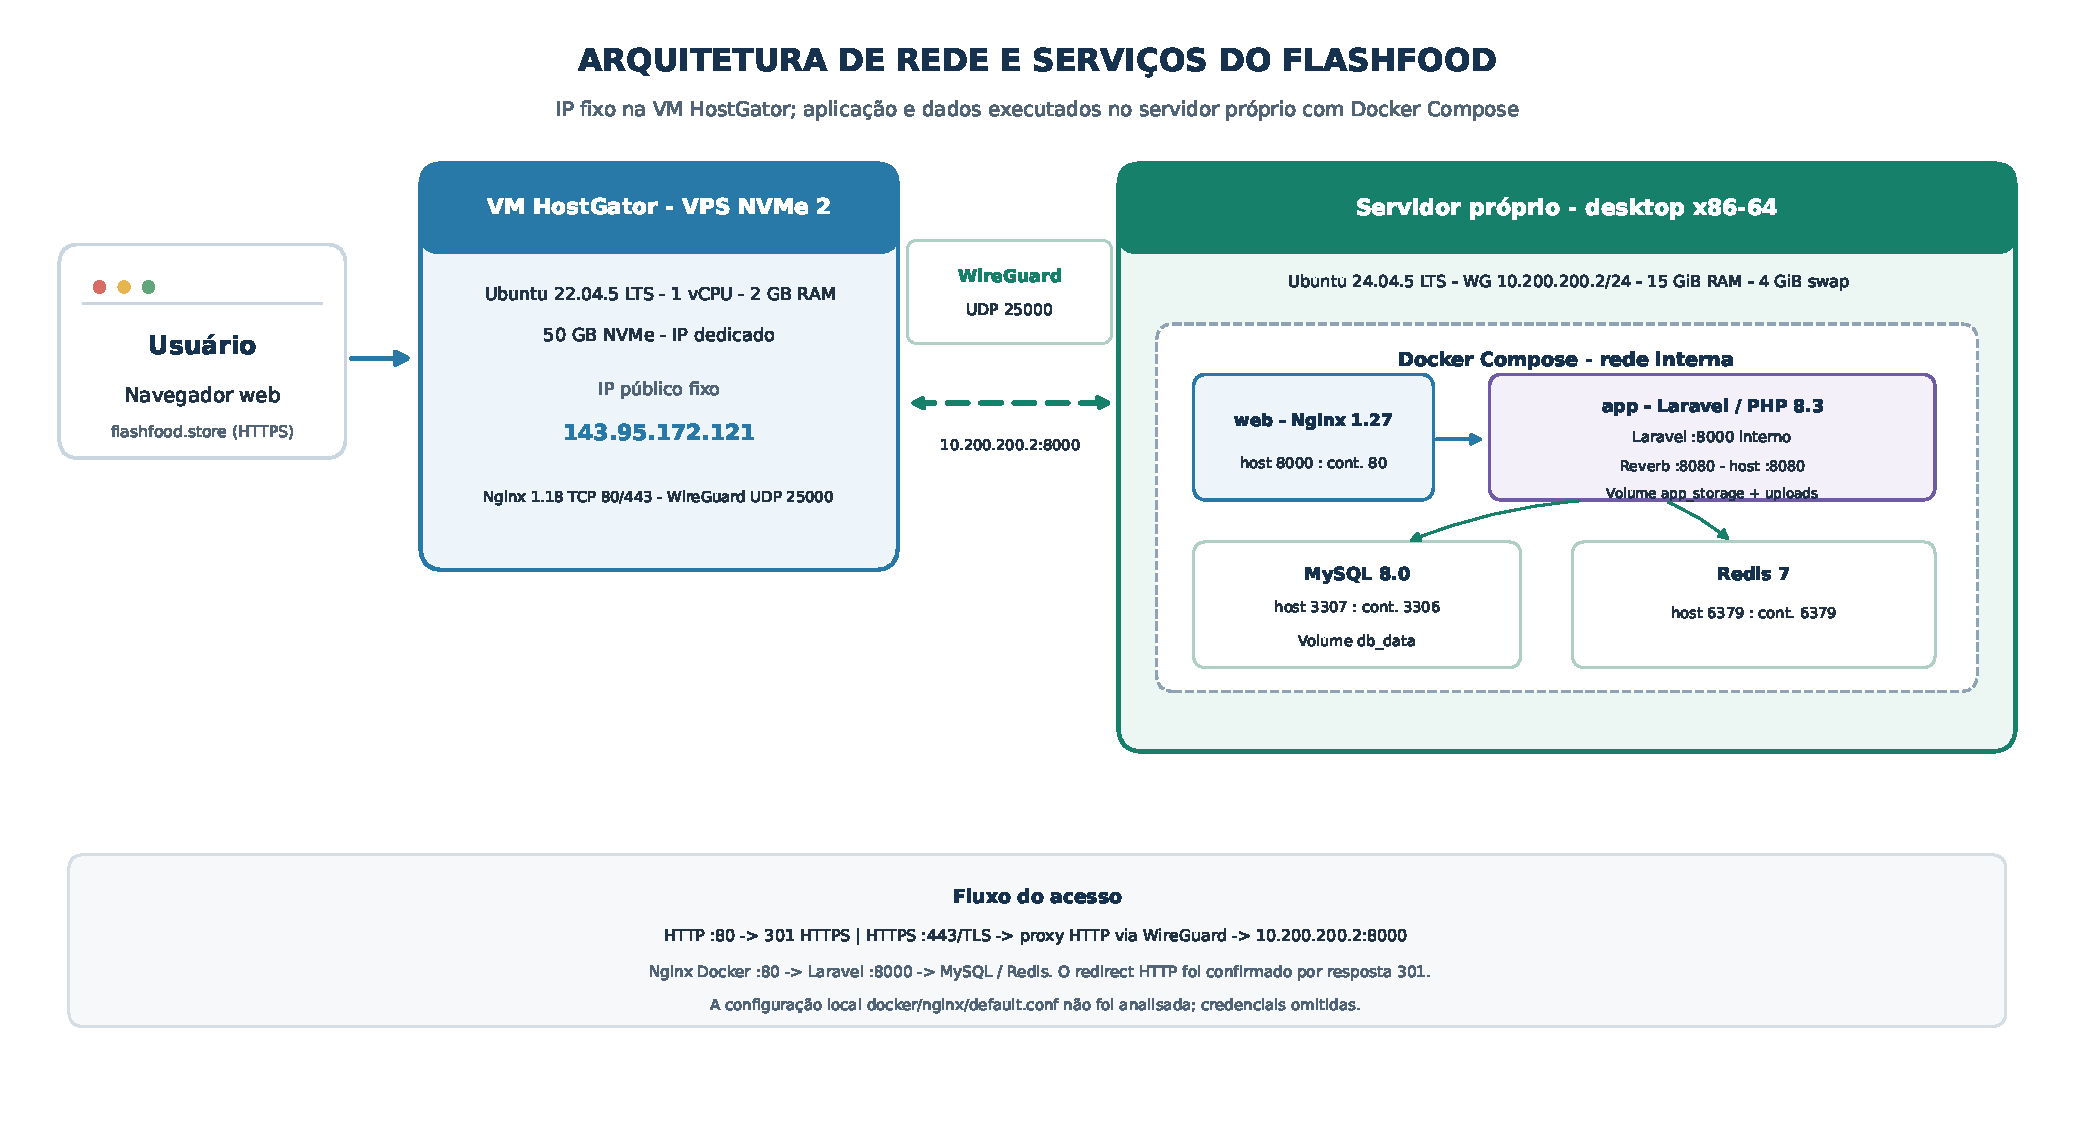
\includegraphics[width=\textwidth]{arquitetura-rede.pdf}
\legend{Elaborado pelo autor (2026)}
\end{figure}

As chaves criptográficas utilizadas para estabelecer a VPN são parâmetros de configuração e não são apresentadas neste trabalho. A descrição registra apenas os endereços da rede privada e a porta de comunicação necessários para caracterizar a arquitetura adotada.
